\subsection{Análisis cualitativo de los métodos}

En esta sección nos concentraremos en las caracteristicas de los métodos utilizados que escapan a nuestros análisis anteriores. Si bien logramos tener una idea de la complejidad temporal y el nivel de error que pueden tener los videos que generamos aun no vimos con suficiente claridad los efectos particulares que pueden llegar a porducirse, qué tipo de errores pueden haber y cómo varian entre los distintos métodos. Esto es de lo que hablaremos en esta sección.

Un video esta formado por una sucesión finita de imagenes, al reproducirlo se pasa de una imagen a la siguiente lo cual puede causar cambios en los valores de los pixels que se estan visualizando. La interpolación se basara en esos pixels para calcular nuevas imagenes que se agregaran al video, en esta sección veremos de que forma el grado de cambio entre los pixels puede afectar la calidad del video resultante tras la interpolación.

Todos los videos sobre los que trabajaremos aquí seran el resultado de aplicar alguno de los métodos de interpolación sobre los pocos videos base que describimos previamente, se detallaran siempre los métodos utilizados de forma que los experimentos realizados puedan replicarse facilmente. Varios de ellos pueden encontrarse en el link citado en la sección del apéndice (\ref{sec:links}).

Nuestra primer hipótesis es que según la forma en que varían los pixels en el video podrían presentarse mayores dificultades y errores al intentar pasarlo a camara lenta. Por lo tanto lo que haremos en esta sección será dividir los experimentos en cuatro tipos de video base y analizar cada caso particular con los métodos propuestos. Escogimos 4 ejemplares distintos, un por cada categoría de video que nos pareció relevante analizar. Para cada video hicimos experimentos con cada método interpolando 1, 2, 4 y 8 cuadros. Se presentarán en esta sección los casos mas representativos de nuestros hallazgos.

\subsubsection{Video de control}

En los próximos experimentos analizaremos videos con movimientos rápidos de objetos y cámara intentando verificar ciertas ideas sobre posibles artifacts que podrian generarse. Antes de eso utilizaremos un video de control el cual no presenta ninguna de esas caracteristicas, este será un video con movimiento relajado el cual nos permitira verificar como se comportan los métodos con videos que, según creemos, no presentaran problemas para luego compararlos con los casos mas problemáticos. El caso mas trivial sería un video completamente estático. Pero se ve facilmente al analizar el funcionamiento de nuestros métodos que el resultado sera un video tambien estático pero de mayor duración, lo cual cumpliría correctamente el resultado deseado. Un caso un poco mas interesante y el cual utilizaremos como video de control es el caso en que hay cierto movimiento pero nada de gran velocidad.

Como video seleccionamos una toma de la carrera de un grupo de babosas.

\begin{figure}[H]
\centering
\begin{minipage}{0.60\textwidth}   
    \fbox{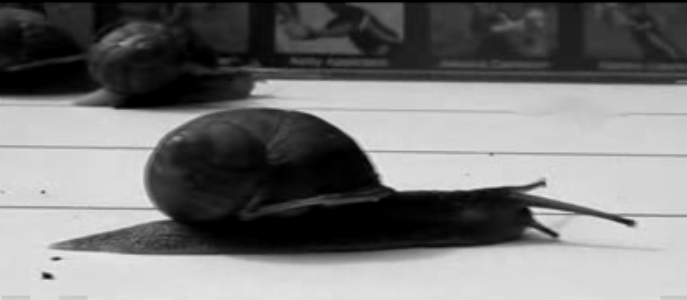
\includegraphics[width=1\textwidth]{imgs/cualitativos/babosa.png}}
\end{minipage}\hfill
\caption{\footnotesize Captura del video babosa.avi con el cuadruple de cuadros de lo normal calculados utilizando splines de bloque de radio 4, no se nota en ningún momento algún artifact significativo.}
\end{figure}

Al ver los resultados se corroboró que utilizando splines y interpolación lineal no habian problemas y el video resultante tenia un buen efecto de camara lenta, solo se notaron partes borrosas en las antenas, creemos que debido a que estas producen los movimientos mas rápidos en el video. Con Nearest Neighbour la historia es distinta, al agregar mas de 2 cuadros al video original comienza a perder mucha fluidés, agregando 8 cuadros el video ya carece completamente de un movimiento natural, esta caracteristica creemos que persistirá siempre al utilizar este método.

\subsubsection{Movimiento rápido de cámara}

Un caso que nos pareció relevante es el de los videos que tienen movimientos rápidos de cámara, como ejemplar de esta situación utilizamos al video nombrado previamente \textit{motocross}. Para este caso volvió a ocurrir con \textit{Nearest Neighbour} que la imagen perdia fluidez a medida que se intentaban agregar mas cuadros. Para  \textit{Splines} e \textit{Interpolación Lineal}  sucedió lo esperado, los movimientos rapidos del video produjeron efectos indeseados, los cuales empeoraban a medida que se agregaban mas cuadros. El error puede observarse en la imagen de la izquierda.

\begin{figure}[H]
\centering
\begin{minipage}{0.48\textwidth}
    \fbox{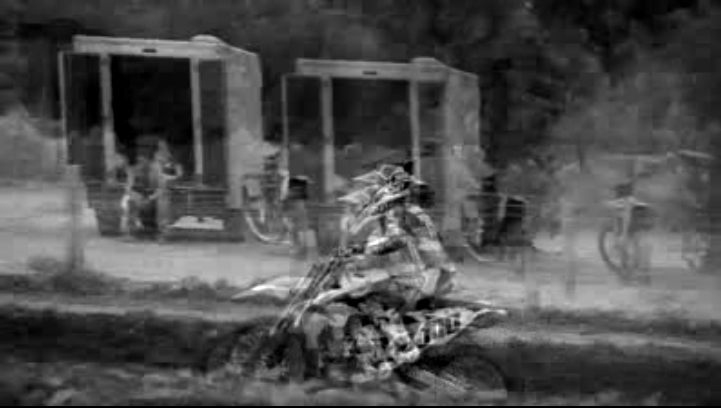
\includegraphics[width=1\textwidth]{imgs/cualitativos/motocross_1.png}}
\end{minipage}%
\hfill
\begin{minipage}{0.48\textwidth}   
    \fbox{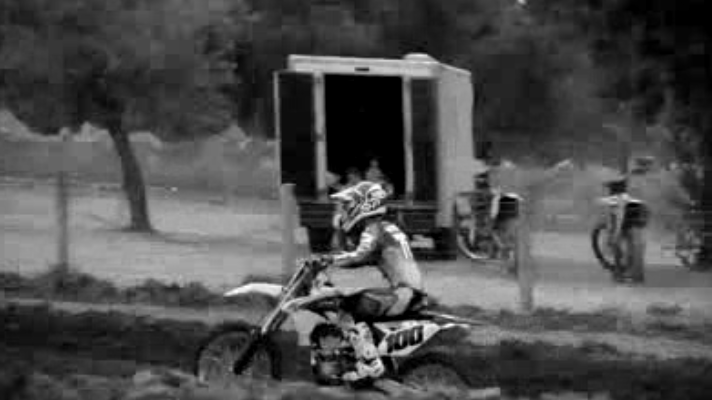
\includegraphics[width=1\textwidth]{imgs/cualitativos/motocross_2.png}}

\end{minipage}
\caption{\footnotesize A la izquierda se tiene el resultado de un cuadro calculado con Splines al interpolar de a 4 cuadros con bloques de radio 4, se observa una superposición importante entre dos imagenes. En la izquierda se ve una toma del video original}
\end{figure}

Lo que sucede es que debido al gran ritmo de cambio entre cada fotograma los cuadros que se agregan al video se calculan basados en imagenes muy distintas, los métodos que utilizamos no son suficientemente buenos para predecir el cuadro adecuado y en concecuencia fallan en dar una imagen intermedia adecuada.

Otra observación que hicimos en este video fue que a simple vista no parece haber diferencia significativa entre los resultados de Splines e interpolación lineal, ambos funcionan correctamente al agregar 1 y 2 cuadros y comienzan a fallar a un ritmo similar al comenzar a agregar mas cuadros. 

\subsubsection{Movimiento rápido de objetos}

Para este experimento utilizamos el video \textit{penal}, este se puede ver como un caso particular del anterior. Ya que hay movimiento rapido de pixels por lo que se presentan los mismos inconvenientes pero solo sobre un pequeño conjunto de pixels, los que estan en la trayectoria de la pelota y el jugador, en ese espacio es donde al utilizar splines y lineal se espera experimentar al igual que en el caso anterior un efecto de transparencia y superposición indeseable entre el fondo y el lugar donde estuvo el objeto previamente.


\begin{figure}[H]
\centering
\begin{minipage}{0.48\textwidth}
    \fbox{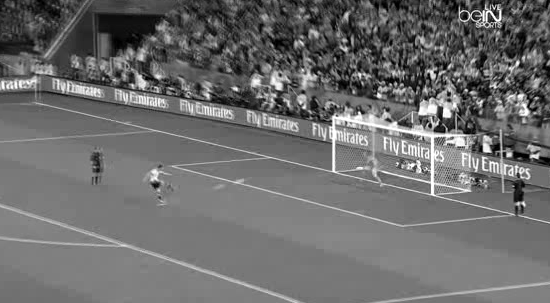
\includegraphics[width=1\textwidth]{imgs/cualitativos/penal_1.png}}
\end{minipage}%
\hfill
\begin{minipage}{0.48\textwidth}   
    \fbox{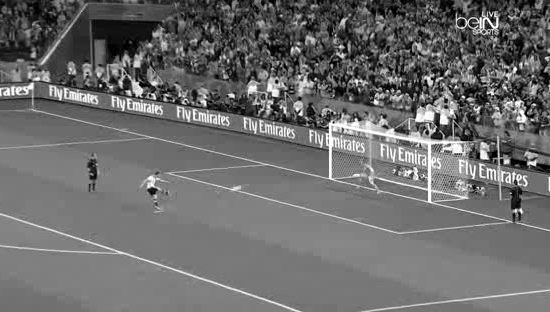
\includegraphics[width=1\textwidth]{imgs/cualitativos/penal_2.png}}

\end{minipage}
\caption{\footnotesize A la izquierda se tiene el resultado de un fotograma calculado con Splines agregando 8 cuadros con bloques de radio 4, se observa una superposición importante entre cuadros. A la derecha esta una toma del video original}
\end{figure}


Al ver los videos se corrobora lo esperado. El artifact visto en la figura aumenta cuanto mayor es la cantidad de cuadros que queremos agregar. Para \textit{Nearest Neighbour} el efecto no existe pero la imagen tiene movimientos muy bruscos y parece mas estática a medida que agregamos mas cuadros.

\subsubsection{Cambio de Cámara}

Los cambios de cámara creemos que serán los que produzcan los mayores problemas para Splines e interpolación lineal debido a que estos producen las mayores diferencias entre cuadros contiguos, creemos que aquí en algunos casos puede llegar a ser preferible incluso \textit{nearest neighbour} a pesar de su dinámica pobre. Para verificar nuestras ideas utilizamos el video \textit{ff6}.
También nos interesa comprobar lo charlado previamente en la sección de errores sobre que tanto afectara el tamaño de los bloques de los Splines, intentaremos ver si esto podria llegar a jugar un rol en que tan dramaticos son los artifacts.


\begin{figure}[H]
\centering
\begin{minipage}{0.31\textwidth}   
    \fbox{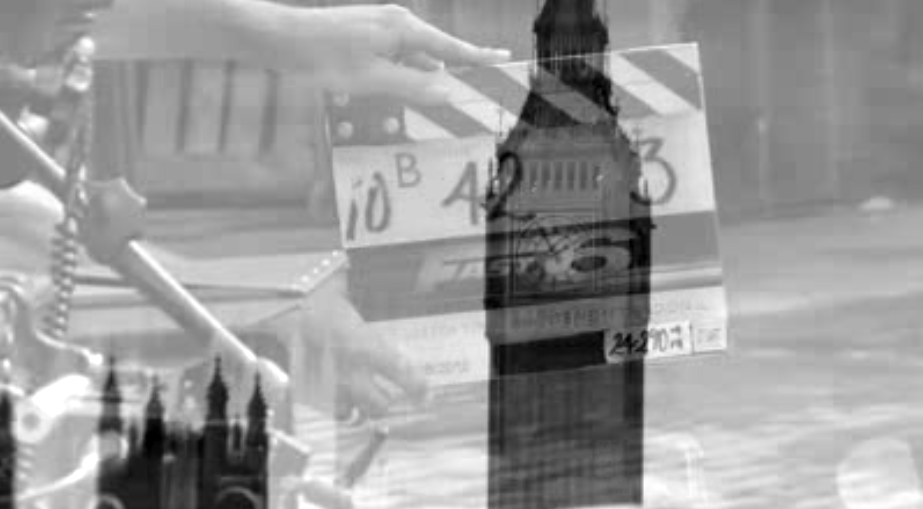
\includegraphics[width=1\textwidth]{imgs/cualitativos/ff6_1.png}}

\end{minipage}
\hfill
\begin{minipage}{0.31\textwidth}   
    \fbox{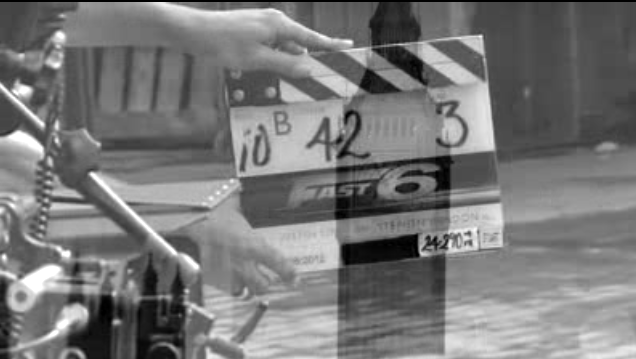
\includegraphics[width=1\textwidth]{imgs/cualitativos/ff6_2.png}}
\end{minipage}
\hfill
\begin{minipage}{0.31\textwidth}   
    \fbox{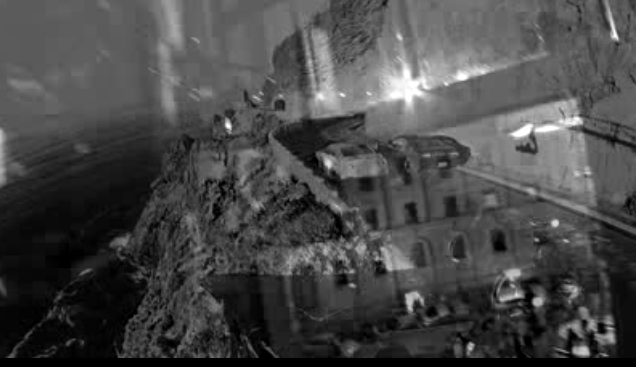
\includegraphics[width=1\textwidth]{imgs/cualitativos/ff6_3.png}}
\end{minipage}
\caption{\footnotesize Distintos artifacts producidos por Splines e Interpolación lineal interpolando 4 cuadros. El del medio es Splines cúbicos interpolando 4 cuadros con 8 de radio, los otros son interpolación lineal de 8 cuadros.}

\label{fig:ff6}

\end{figure}

\begin{figure}[H]
\centering
\begin{minipage}{0.31\textwidth}   
    \fbox{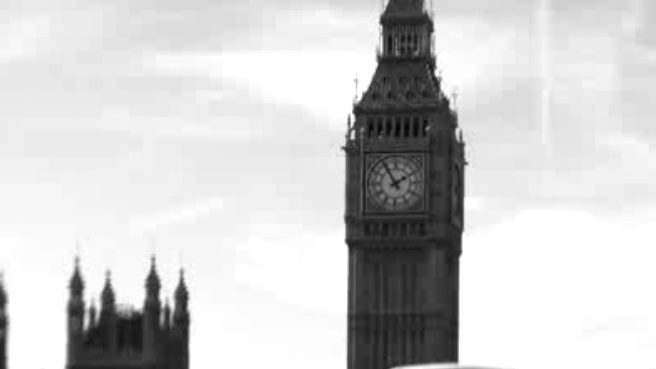
\includegraphics[width=1\textwidth]{imgs/cualitativos/ff6_4.png}}

\end{minipage}
\hfill
\begin{minipage}{0.31\textwidth}   
    \fbox{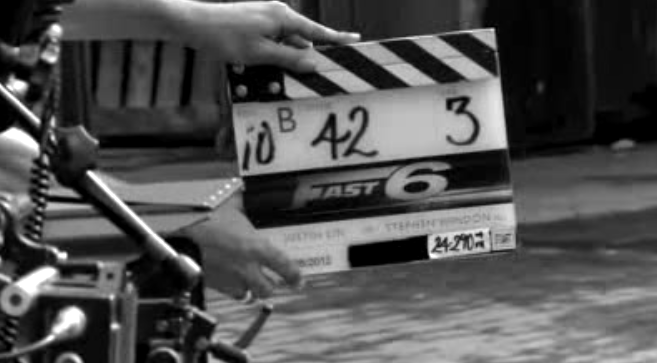
\includegraphics[width=1\textwidth]{imgs/cualitativos/ff6_7.png}}
\end{minipage}
\hfill
\begin{minipage}{0.31\textwidth}   
    \fbox{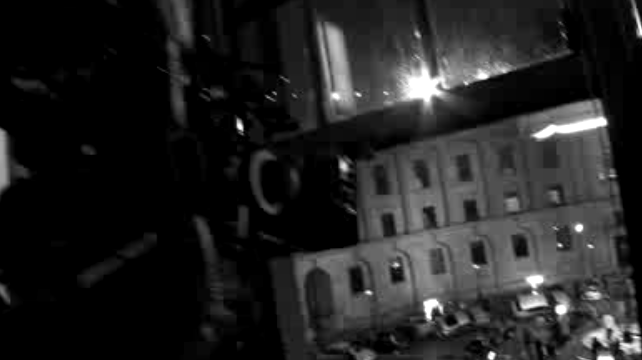
\includegraphics[width=1\textwidth]{imgs/cualitativos/ff6_6.png}}
\end{minipage}
\caption{\footnotesize Imagenes originales.}

\label{fig:ff6}

\end{figure}

Como se ve en las imagenes hay cuadros formados por imagenes totalmente distintas fusionadas lo cual produce un efecto indeseable. Estos problemas se ven a lo largo de todos los cambios de cámara del video. Se deduce de este experimento que no es buena idea intentar interpolar entre cambios de cámara, una posible solución podria ser trabajar sobre cada toma por separado, hacer la interpolación deseada y luego volver a unir los subvideos obtenidos, asi se evitaria generar cuadros entre tomas de lugares distintos.

Con respecto al tamaño de los bloques de Splines se pudo verificar lo charlado anteriormente en la sección de errores, con distintos tamaños de bloque (se utilizaron radios de 1, 2, 8 y 16) no se observaron cambios significativos.

Como observación final debemos decir que a simple vista no pudimos presenciar para ninguno de los casos analizados una diferencia demasiado abrupta entre interpolación lineal y Splines con distintos tamaños de bloques. Si bien en ciertas circunstancias habian mejoras con algunos de estos métodos respecto de los demás estas no superaban ampliamente a las demas y presentaban los mismos artifacts y decadencias para casos iguales de interpolación. Esta observación de seguro este relacionada con la calidad baja de los videos y la impresición del análisis a ojo por lo que quedara como trabajo a futuro la verificación y profundización de esta idea.
